%MKB
%Mathematik
%Übungseinheit 3
%Hausübungen
%Aufgabe P5

\setcounter{P-section}{5}
\renewcommand*\thesection{P\Nummerierung{\arabic{P-section}}}
\section{Analyse einiger Kavalierprojektionen}

%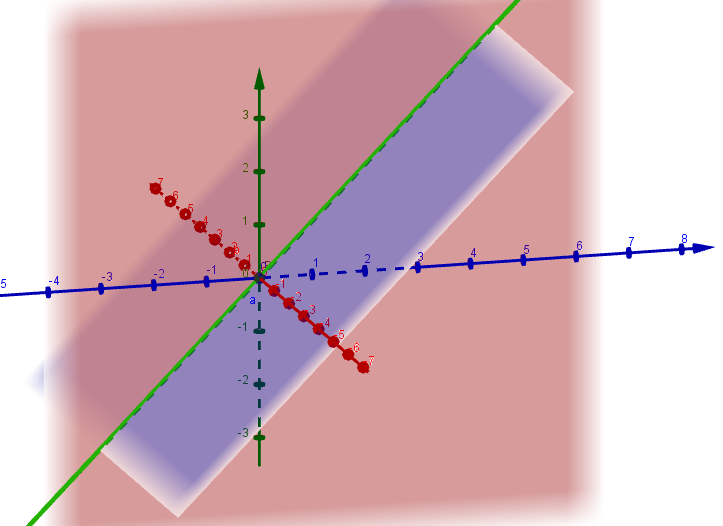
\includegraphics[scale = .8]{MKB/UE_03/Schnittgerade.png}\\

\begin{minipage}{\linewidth}
	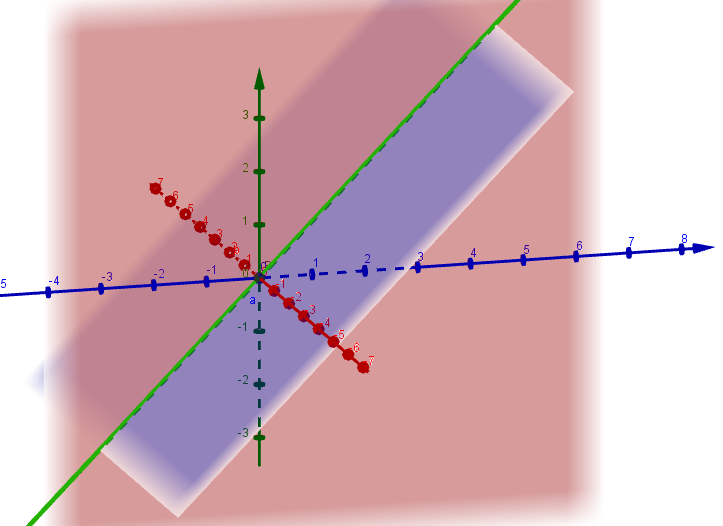
\includegraphics[width=1.\linewidth]{MKB/UE_03/Schnittgerade.png}
		\captionof{figure}{Rote Ebene = Bildebene \ensuremath{(x_2 = x_3)}, blaue Ebene = Menge der möglichen Projektionsgeraden \ensuremath{(x_1 = 0)}, grüne Gerade = Schnittgerade der beiden Ebenen diese bezeichnen wir als die Menge aller möglichen Punkte \ensuremath{E_1'}. Rote Achse = \ensuremath{E_1}, blaue Achse = \ensuremath{E_3}, grüne Achse = \ensuremath{E_2} }
\end{minipage}


\begin{center}
	\begin{tikzpicture}[x=2cm,y=2cm,z=1.414cm,>=stealth]
	
	\draw[step=2cm,lightgray,very thin,dashed] (0,2.5) grid (2.5,0);
	
	% The axes
	\draw[->] (xyz cs:x=-1.5) -- (xyz cs:x=2.5) node[above] {$E_2$};
	\draw[->] (xyz cs:y=-1.5) -- (xyz cs:y=2.5) node[right] {$E_3$};
	\draw[->] (xyz cs:z=-1.5) -- (xyz cs:z=2.5) node[above] {$E_1$};
	% The thin ticks
	
	\foreach \coo in {-1,0,...,2}
	{
		\draw (\coo,-1.5pt) -- (\coo,1.5pt);
		\draw (-1.5pt,\coo) -- (1.5pt,\coo);
		%\draw (xyz cs:y=-0.15pt,z=\coo) -- (xyz cs:y=0.15pt,z=\coo);
	}
	
	% The thick ticks
	\foreach \coo in {1}
	{
		\draw[thick] (\coo,-0.5pt) -- (\coo,0.5pt) node[below=6pt] {\coo};
		\draw[thick] (-0.5pt,\coo) -- (0.5pt,\coo) node[left=6pt] {\coo};
		\draw[thick] (xyz cs:y=-0.03pt,z=\coo) -- (xyz cs:y=0.02pt,z=\coo) node[below=8pt] {\coo};
	}
	
	%Wall back
	\fill[red] (xyz cs:x=0,y=0,z=1) circle(4pt);
	\draw[red] (xyz cs:x=0,y=0,z=1)--+(0,-0.707,0)node[below]{$x$};
	\draw[red] (xyz cs:x=0,y=0,z=1)--+(-0.707,0,0)node[left]{$x$};

	\end{tikzpicture}
\end{center}
\begin{gather}
1=\sqrt{x^2+x^2}\\
1=\sqrt{2} \cdot x\\
x = \frac{1}{\sqrt{2}}\\
s_1'=\begin{pmatrix}
0\\\frac{1}{\sqrt{2}}\\\frac{1}{\sqrt{2}}
\end{pmatrix}	
\end{gather}

\begin{center}
	\begin{tikzpicture}[x=2cm,y=2cm,z=1.414cm,>=stealth]
	
	\draw[step=2cm,lightgray,very thin,dashed] (0,2.5) grid (2.5,0);
	
	% The axes
	\draw[->] (xyz cs:x=-1.5) -- (xyz cs:x=2.5) node[above] {$E_1$};
	\draw[->] (xyz cs:y=-1.5) -- (xyz cs:y=2.5) node[right] {$E_1'$};
%	\draw[->] (xyz cs:z=-1.5) -- (xyz cs:z=2.5) node[above] {$E_1$};
	% The thin ticks
	
	\foreach \coo in {-1,0,...,2}
	{
		\draw (\coo,-1.5pt) -- (\coo,1.5pt);
		\draw (-1.5pt,\coo) -- (1.5pt,\coo);
		%\draw (xyz cs:y=-0.15pt,z=\coo) -- (xyz cs:y=0.15pt,z=\coo);
	}

	\draw[red] (xyz cs:x=1,y=0)node[below]{$E_1$}--(xyz cs:x=0,y=1) node[left]{$E_1'$};
	
	\node[align=center] at (0.4,0.4) (ori) {\text{45$\circ$}};
	\draw[->,help lines,shorten >=3pt] (ori) .. controls (0.4,0.4) and (0.4,0.4) .. (0,1,0);
	
	\end{tikzpicture}
\end{center}

\begin{gather}
	s_1 = \overline{OE_1'}\\
	 s_1 \coloneqq 1
\end{gather}

b)

\begin{center}
	\begin{tikzpicture}[x=2cm,y=2cm,z=1.414cm,>=stealth]
	
	\draw[step=2cm,lightgray,very thin,dashed] (0,2.5) grid (2.5,0);
	
	% The axes
	\draw[->] (xyz cs:x=-1.5) -- (xyz cs:x=2.5) node[above] {$E_1$};
	\draw[->] (xyz cs:y=-1.5) -- (xyz cs:y=2.5) node[right] {$E_1'$};
	%	\draw[->] (xyz cs:z=-1.5) -- (xyz cs:z=2.5) node[above] {$E_1$};
	% The thin ticks
	
	\foreach \coo in {-1,0,...,2}
	{
		\draw (\coo,-1.5pt) -- (\coo,1.5pt);
		\draw (-1.5pt,\coo) -- (1.5pt,\coo);
		%\draw (xyz cs:y=-0.15pt,z=\coo) -- (xyz cs:y=0.15pt,z=\coo);
	}
	
	\draw[red] (xyz cs:x=1,y=0)node[below]{$E_1$}--(xyz cs:x=0,y=2) node[left]{$E_1'$};
	
	\node[align=center] at (0.4,0.4) (ori) {\text{45$\circ$}};
	\draw[->,help lines,shorten >=3pt] (ori) .. controls (0.4,0.4) and (0.4,0.4) .. (0,2,0);
	
	\end{tikzpicture}
\end{center}

\begin{gather}
s_1 = \overline{OE_1'}\\
s_1 \coloneqq 2\\
\tan(\delta)=\frac{\textbf{Gegenkathete}}{\textbf{Ankathete}}\\
\delta= \tan^{-1}\Big(\frac{1}{2}\Big)\\
\delta = 26.57^\circ
\end{gather}

c)\\

\begin{center}
	\begin{tikzpicture}[x=2cm,y=2cm,z=1.414cm,>=stealth]
	
	\draw[step=4cm,lightgray,very thin,dashed] (0,2.5) grid (2.5,0);
	
	% The axes
	\draw[->] (xyz cs:x=-1.5) -- (xyz cs:x=2.5) node[above] {$E_1$};
	\draw[->] (xyz cs:y=-1.5) -- (xyz cs:y=2.5) node[right] {$E_1'$};
	%	\draw[->] (xyz cs:z=-1.5) -- (xyz cs:z=2.5) node[above] {$E_1$};
	% The thin ticks
	
	\foreach \coo in {-1,0,...,2}
	{
		\draw (\coo,-1.5pt) -- (\coo,1.5pt);
		\draw (-1.5pt,\coo) -- (1.5pt,\coo);
		%\draw (xyz cs:y=-0.15pt,z=\coo) -- (xyz cs:y=0.15pt,z=\coo);
	}
	
	\draw[red] (xyz cs:x=1,y=0)node[below]{$E_1$}--(xyz cs:x=0,y=0.5) node[left]{$E_1'$};
	
	\node[align=center] at (0.4,0.4) (ori) {\text{45$\circ$}};
	\draw[->,help lines,shorten >=3pt] (ori) .. controls (0.4,0.4) and (0.4,0.4) .. (0,0.5,0);
	
	\end{tikzpicture}
\end{center}

\begin{gather}
s_1 = \overline{OE_1'}\\
s_1 \coloneqq \frac{1}{2}\\
\tan(\delta)=\frac{\textbf{Gegenkathete}}{\textbf{Ankathete}}\\
\delta= \tan^{-1}\Big(\frac{2}{1}\Big)\\
\delta = 63.43^\circ
\end{gather}

d)\\
\begin{center}
	\begin{tikzpicture}[x=2cm,y=2cm,z=1.414cm,>=stealth]
	
	\draw[step=4cm,lightgray,very thin,dashed] (0,2.5) grid (2.5,0);
	
	% The axes
	\draw[->] (xyz cs:x=-1.5) -- (xyz cs:x=2.5) node[above] {$E_1$};
	\draw[->] (xyz cs:y=-1.5) -- (xyz cs:y=2.5) node[right] {$E_1'$};
	%	\draw[->] (xyz cs:z=-1.5) -- (xyz cs:z=2.5) node[above] {$E_1$};
	% The thin ticks
	
	\foreach \coo in {-1,0,...,2}
	{
		\draw (\coo,-1.5pt) -- (\coo,1.5pt);
		\draw (-1.5pt,\coo) -- (1.5pt,\coo);
		%\draw (xyz cs:y=-0.15pt,z=\coo) -- (xyz cs:y=0.15pt,z=\coo);
	}
	
	\draw[red] (xyz cs:x=1,y=0)node[below]{$E_1$}--(xyz cs:x=0,y=0.707) node[left]{$E_1'$};
	
	\node[align=center] at (0.2,0.2) (ori) {\text{45$\circ$}};
	\draw[->,help lines,shorten >=3pt] (ori) .. controls (0.3,0.3
	) and (0.4,0.4) .. (0,0.707,0);
	
	\end{tikzpicture}
\end{center}

\begin{gather}
s_1 = \overline{OE_1'}\\
s_1 \coloneqq \frac{\sqrt{2}}{2}\\
\tan(\delta)=\frac{\textbf{Gegenkathete}}{\textbf{Ankathete}}\\
\delta= \tan^{-1}\Big(\frac{2}{\sqrt{2}}\Big)\\
\delta = 54.74 ^\circ
\end{gather}